\documentclass[conference,a4paper]{IEEEtran}
\usepackage[T1]{fontenc}
\usepackage{cite}
\usepackage{amsmath,amssymb}
\usepackage{graphicx}
\usepackage{booktabs}
\usepackage{array}
\usepackage{url}
\def\UrlBreaks{\do\/\do\-\do\.\do\_\do\:}
\Urlmuskip=0mu plus 2mu
\usepackage{tikz}
\usetikzlibrary{arrows.meta,positioning,calc}
\usepackage{textcomp}
\def\BibTeX{{\rm B\kern-.05em{\sc i\kern-.025em b}\kern-.08em T\kern-.1em\lower.7ex\hbox{E}\kern-.125em X}}

\tikzset{
  blk/.style={draw,rounded corners=1pt,minimum height=0.75cm,minimum width=1.9cm,align=center,font=\scriptsize,thick},
  st/.style={draw,rounded corners=2pt,minimum height=0.8cm,minimum width=3.1cm,align=center,font=\scriptsize\ttfamily,thick},
  arr/.style={-{Stealth[length=2mm]},thick},
  lab/.style={font=\scriptsize\itshape,fill=white,inner sep=1pt}
}

\emergencystretch=2em
\begin{document}

%%%%%%%%%%%%%%%%%%%% COVER PAGE %%%%%%%%%%%%%%%%%%%%
\onecolumn
\pagestyle{empty}
\begin{center}
\vspace*{0.6cm}
{\Large\bfseries Newton School of Technology}\\[3pt]
{\large Rishihood University}\\[2pt]
{\normalsize Sonipat, Haryana, India}\\[0.5cm]
\rule{\textwidth}{0.8pt}\\[0.9cm]
{\LARGE\bfseries Design and Implementation of a\\[4pt] Direct-Mapped Cache Controller}\\[0.7cm]
{\large Phase I Project Report}\\[0.9cm]
\rule{0.5\textwidth}{0.4pt}\\[0.7cm]
{\large\textbf{Project Title:} Direct-Mapped Cache Controller}\\[6pt]
{\large\textbf{Team Name:} 5bit registers \qquad \textbf{Section:} C}\\[1.0cm]
{\large\bfseries Team Members}\\[0.4cm]
\renewcommand{\arraystretch}{1.7}
\begin{tabular}{|l|c|l|}
\hline
\textbf{Name} & \textbf{Enrollment No.} & \textbf{Email}\\ \hline
Krishna & 2401010237 & \texttt{krishna.2024@nst.rishihood.edu.in}\\ \hline
Aditya Rana & 2401010034 & \texttt{aditya.rana2024@nst.rishihood.edu.in}\\ \hline
Rachit Gupta & 2401010363 & \texttt{rachit.gupta2024@nst.rishihood.edu.in}\\ \hline
Saumya Mishra & 2401020057 & \texttt{saumya.mishra2024@nst.rishihood.edu.in}\\ \hline
Nishtha Gupta & 2401010303 & \texttt{nishtha.gupta2024@nst.rishihood.edu.in}\\ \hline
\end{tabular}\\[1.2cm]
{\large 14 November 2026}
\end{center}
\clearpage

%%%%%%%%%%%%%%%%%%%% INDEX %%%%%%%%%%%%%%%%%%%%
\pagestyle{plain}
\pagenumbering{roman}
\begin{center}{\Large\bfseries Index}\end{center}
\vspace{0.1cm}
\renewcommand{\arraystretch}{1.0}
\small
\noindent\begin{tabular}{@{}p{1.2cm}p{12cm}r@{}}
 & Abstract and Index Terms & \pageref{sec:abs}\\
I. & Introduction & \pageref{sec:intro}\\
II. & Literature Review & \pageref{sec:lit}\\
III. & Proposed Solution & \pageref{sec:sol}\\
 & \hspace{1em}A. System Architecture & \pageref{sec:arch}\\
 & \hspace{1em}B. Cache Organization and Address Mapping & \pageref{sec:map}\\
 & \hspace{1em}C. Read and Write Operation & \pageref{sec:rw}\\
 & \hspace{1em}D. Controller Microarchitecture & \pageref{sec:fsm}\\
IV. & Implementation & \pageref{sec:impl}\\
 & \hspace{1em}A. Module Hierarchy & \pageref{sec:mods}\\
 & \hspace{1em}B. Main-Memory Model and Performance Monitor & \pageref{sec:memmon}\\
 & \hspace{1em}C. Top-Level Interface & \pageref{sec:iface}\\
V. & Verification and Results & \pageref{sec:ver}\\
 & \hspace{1em}A. Verification Methodology & \pageref{sec:meth}\\
 & \hspace{1em}B. Unit-Level Results & \pageref{sec:unit}\\
 & \hspace{1em}C. Integrated Results and Waveform Scenarios & \pageref{sec:integ}\\
 & \hspace{1em}D. Waveform Timing Analysis & \pageref{sec:wave}\\
 & \hspace{1em}E. Integrated Access Trace & \pageref{sec:trace}\\
 & \hspace{1em}F. Requirements Traceability & \pageref{sec:trace2}\\
VI. & Performance Analysis & \pageref{sec:perf}\\
 & \hspace{1em}A. Hit and Miss Rates & \pageref{sec:hit}\\
 & \hspace{1em}B. Measured Completion Latency & \pageref{sec:lat}\\
 & \hspace{1em}C. Average Access Time & \pageref{sec:amat}\\
 & \hspace{1em}D. Trace-Driven Benchmark & \pageref{sec:bench}\\
VII. & Discussion and Limitations & \pageref{sec:disc}\\
VIII. & Alternative Organizations and Synthesis Results & \pageref{sec:alt}\\
IX. & Individual Contributions & \pageref{sec:contrib}\\
X. & Conclusion and Future Work & \pageref{sec:concl}\\
 & Appendix A: Reproducing the Results & \pageref{app:repro}\\
 & References & \pageref{sec:refs}\\
\end{tabular}

\vspace{0.3cm}
\noindent\textbf{List of Figures}\\[2pt]
\begin{tabular}{@{}p{1.6cm}p{11.6cm}r@{}}
Fig.~\ref{fig:arch} & Block-level architecture of the integrated direct-mapped cache & \pageref{fig:arch}\\
Fig.~\ref{fig:addr} & 32-bit byte-address partition used by the decoder & \pageref{fig:addr}\\
Fig.~\ref{fig:fsm} & Controller FSM paths & \pageref{fig:fsm}\\
Fig.~\ref{fig:wavehit} & Waveform: cold read miss followed by a read hit & \pageref{fig:wavehit}\\
Fig.~\ref{fig:wavewt} & Waveform: write hit, write miss and read hit & \pageref{fig:wavewt}\\
Fig.~\ref{fig:amat} & Analytical average read latency versus hit rate & \pageref{fig:amat}\\
Fig.~\ref{fig:bench} & Analytical and measured AMAT for the benchmark workloads & \pageref{fig:bench}\\
\end{tabular}

\vspace{0.2cm}
\noindent\textbf{List of Tables}\\[2pt]
\begin{tabular}{@{}p{1.6cm}p{11.6cm}r@{}}
Table~\ref{tab:cfg} & Cache configuration & \pageref{tab:cfg}\\
Table~\ref{tab:ex} & Worked address-decoding examples & \pageref{tab:ex}\\
Table~\ref{tab:states} & Controller states and actions & \pageref{tab:states}\\
Table~\ref{tab:mods} & RTL modules and source files & \pageref{tab:mods}\\
Table~\ref{tab:ports} & \texttt{cache\_top} ports & \pageref{tab:ports}\\
Table~\ref{tab:unit} & Unit-level verification results & \pageref{tab:unit}\\
Table~\ref{tab:scen} & Isolated waveform scenarios & \pageref{tab:scen}\\
Table~\ref{tab:cnt} & Performance counters: expected vs.\ actual & \pageref{tab:cnt}\\
Table~\ref{tab:trace} & Classified access trace of the integrated sequence & \pageref{tab:trace}\\
Table~\ref{tab:req} & Requirement-to-evidence mapping & \pageref{tab:req}\\
Table~\ref{tab:lat} & Measured completion latency per access type & \pageref{tab:lat}\\
Table~\ref{tab:traces} & Benchmark workloads and simulated hit/miss counts & \pageref{tab:traces}\\
Table~\ref{tab:bench} & Trace benchmark results (analytical estimates) & \pageref{tab:bench}\\
\end{tabular}
\normalsize
\clearpage

%%%%%%%%%%%%%%%%%%%% PAPER %%%%%%%%%%%%%%%%%%%%
\pagenumbering{arabic}
\twocolumn
\title{Design and Implementation of a Direct-Mapped Cache Controller}
\author{%
\IEEEauthorblockN{Krishna}
\IEEEauthorblockA{\textit{Enroll. No.\ 2401010237}\\ krishna.2024@nst.rishihood.edu.in}
\and
\IEEEauthorblockN{Aditya Rana}
\IEEEauthorblockA{\textit{Enroll. No.\ 2401010034}\\ aditya.rana2024@nst.rishihood.edu.in}
\and
\IEEEauthorblockN{Rachit Gupta}
\IEEEauthorblockA{\textit{Enroll. No.\ 2401010363}\\ rachit.gupta2024@nst.rishihood.edu.in}
\and
\IEEEauthorblockN{Saumya Mishra}
\IEEEauthorblockA{\textit{Enroll. No.\ 2401020057}\\ saumya.mishra2024@nst.rishihood.edu.in}
\and
\IEEEauthorblockN{Nishtha Gupta}
\IEEEauthorblockA{\textit{Enroll. No.\ 2401010303}\\ nishtha.gupta2024@nst.rishihood.edu.in}
\and
\IEEEauthorblockN{Team ``5bit registers'', Section C}
\IEEEauthorblockA{\textit{Newton School of Technology, Rishihood University}\\ Sonipat, Haryana, India}
}
\maketitle

\begin{abstract}\label{sec:abs}
This paper presents the design and Phase~I verification of a 32-bit direct-mapped cache subsystem that reduces average memory-access latency by exploiting temporal and spatial locality. The cache holds 1~KiB as 64 lines of 16-byte blocks (four 32-bit words per line), with a 22-bit tag, 6-bit index and 4-bit offset, and uses write-through and write-allocate policies. The modular Verilog RTL comprises an address decoder, cache storage, an FSM controller, a behavioral main-memory model and a performance monitor. Verification records 374 decoder checks, unit tests for every module, and 39 integrated checks passing with no failures over a 26-access directed sequence (13 hits, 13 misses), supported by eight waveform scenarios. Waveform measurements give completion latencies of 2, 11, 9 and 18 cycles for a read hit, read miss, write hit and write miss. Four read workloads replayed through the RTL give hit rates of 80\% (sequential), 93.75\% (repeated block), 0\% (conflict thrashing) and 35.9\% (seeded random), with measured average memory access times of 3.80, 2.56, 11.00 and 7.77 cycles; a Python model of the same mapping reproduces every hit and miss count. Synthesized for a Lattice ECP5-85F, the cache uses 18{,}851 LUTs, 10{,}978 flip-flops and one block RAM and closes timing at 61.1~MHz after place-and-route.
\end{abstract}

\begin{IEEEkeywords}
Cache memory, direct mapping, cache controller, Verilog HDL, write-through, write-allocate, finite-state machine, memory hierarchy.
\end{IEEEkeywords}

%%%%%%%%%%%%%%%%%%%% I %%%%%%%%%%%%%%%%%%%%
\section{Introduction}\label{sec:intro}
The processor--memory performance gap motivates the use of cache memory: a small, fast storage structure placed between a processor and a larger, slower main memory. Caches exploit \emph{temporal locality}, in which recently accessed data is likely to be accessed again, and \emph{spatial locality}, in which nearby addresses are likely to be accessed soon. A cache keeps recently used memory blocks so that subsequent requests can be served without accessing main memory \cite{patterson,arm}.

This project develops a modular direct-mapped cache subsystem in Verilog HDL \cite{verilog}. In direct mapping, each main-memory block is assigned to exactly one cache line. The line index selects the candidate line, while a stored tag and a valid bit determine whether the requested block is present \cite{patterson,arm}. Direct mapping offers a simple lookup and replacement mechanism, although blocks that map to the same line can evict one another.

The Phase~I objectives are to (i)~specify the microarchitecture and the interface contract between modules, (ii)~develop modular RTL, (iii)~verify functional behavior with directed self-checking testbenches, (iv)~expose hardware counters that classify every completed processor access as a hit or a miss, and (v)~evaluate locality and conflict behavior with a reproducible trace-driven benchmark. The remainder of this paper is organized as follows. Section~\ref{sec:lit} reviews background literature, Section~\ref{sec:sol} describes the proposed architecture, Section~\ref{sec:impl} details the implementation and its interfaces, Section~\ref{sec:ver} reports verification results including waveform timing, Section~\ref{sec:perf} analyzes performance from measured latencies and a trace-driven benchmark, Section~\ref{sec:disc} discusses design decisions and limitations, and Sections~\ref{sec:alt}--\ref{sec:concl} cover alternatives, contributions and conclusions. Appendix~\ref{app:repro} explains how to reproduce the results.

%%%%%%%%%%%%%%%%%%%% II %%%%%%%%%%%%%%%%%%%%
\section{Literature Review}\label{sec:lit}
Classical computer-architecture literature describes cache organization in terms of placement, identification and replacement \cite{patterson,hennessy}. In a direct-mapped organization, the index selects one line and the tag comparison determines whether that line contains the requested memory block. Only one tag comparison is required, which simplifies both lookup and replacement logic \cite{patterson}.

Arm's architecture documentation explains that a direct-mapped cache maps each main-memory location to one cache location. The address is divided into tag, index and offset fields: the index chooses a line, the tag identifies the resident block, and the offset selects the requested data within the block \cite{arm}. The IIT Kharagpur Virtual Labs compare direct-mapped, fully associative and set-associative organizations; direct mapping is straightforward because each memory block has one permitted location, but its rigid placement can cause \emph{conflict misses} when frequently used blocks compete for the same line \cite{iitkgp}.

Standard write policies include \emph{write-through}, in which a write updates both the cache and the next memory level, and \emph{write-back}, in which modified data may remain in the cache until eviction \cite{hennessy}. This project uses write-through to keep main memory consistent with cache contents and \emph{write-allocate} to fetch a block on a write miss before updating the selected word. The combination removes the need for dirty bits and simplifies the prototype, at the cost of requiring memory completion for every write.

%%%%%%%%%%%%%%%%%%%% III %%%%%%%%%%%%%%%%%%%%
\section{Proposed Solution}\label{sec:sol}
The proposed system is a 1~KiB, 32-bit, direct-mapped cache with 64 lines and 16-byte blocks. Each line holds a valid bit, a 22-bit tag and 128 data bits (four 32-bit words). The address decoder extracts the tag, line index and word offset. Cache storage holds tags, valid bits and data blocks. The controller coordinates processor requests, cache lookups, refills, writes and memory handshakes. The performance monitor counts completed processor accesses and classifies them as hits or misses. Table~\ref{tab:cfg} summarizes the configuration.

\begin{table}[!t]
\caption{Cache Configuration}\label{tab:cfg}
\centering
\renewcommand{\arraystretch}{1.1}
\begin{tabular}{@{}ll@{}}
\toprule
\textbf{Parameter} & \textbf{Value}\\
\midrule
Address width & 32 bits (byte addressed)\\
Capacity & 1 KiB (1024 bytes)\\
Mapping & Direct-mapped\\
Lines $\times$ block size & $64 \times 16$ bytes\\
Words per line & 4 $\times$ 32-bit\\
Tag / index / offset & 22 / 6 / 4 bits\\
Access granularity & Aligned 32-bit words\\
Write policy & Write-through, write-allocate\\
Main-memory latency (model) & 5 cycles (configurable)\\
\bottomrule
\end{tabular}
\end{table}

\subsection{System Architecture}\label{sec:arch}
Fig.~\ref{fig:arch} shows the logical module hierarchy. The processor interface supplies a request, an operation type, an address and write data. The controller latches an accepted request and uses the decoder and cache storage for lookup. On a miss, it requests a 16-byte block from main memory; on writes, it propagates the selected 32-bit word to memory. Completion events are counted by the performance monitor.

\begin{figure}[!t]
\centering
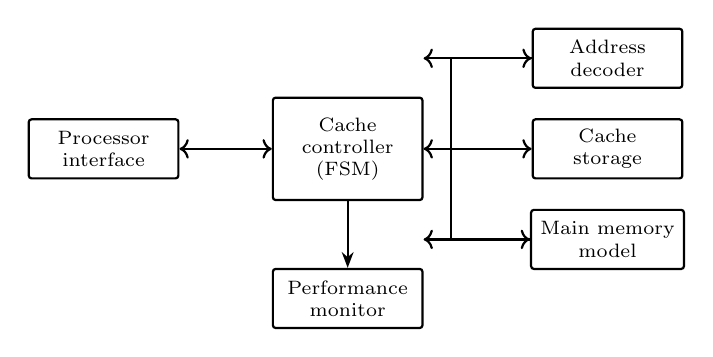
\begin{tikzpicture}
\node[blk] (cpu) at (0,0) {Processor\\interface};
\node[blk,minimum height=1.3cm] (ctl) at (3.1,0) {Cache\\controller\\(FSM)};
\node[blk] (dec) at (6.4,1.15) {Address\\decoder};
\node[blk] (sto) at (6.4,0) {Cache\\storage};
\node[blk] (mem) at (6.4,-1.15) {Main memory\\model};
\node[blk] (pm) at (3.1,-1.9) {Performance\\monitor};
\draw[arr,<->] (cpu) -- (ctl);
\draw[arr,<->] (ctl.east |- dec) -- (dec);
\draw[arr,<->] (ctl) -- (sto);
\draw[arr,<->] (ctl.east |- mem) -- (mem);
\draw[arr] (ctl.south) -- (pm.north);
\draw[thick] (ctl.east) -- ++(0.35,0) |- (dec.west);
\draw[thick] (ctl.east) -- ++(0.35,0) |- (mem.west);
\end{tikzpicture}
\caption{Block-level architecture of the integrated direct-mapped cache.}\label{fig:arch}
\end{figure}

\subsection{Cache Organization and Address Mapping}\label{sec:map}
The cache capacity is 1024 bytes. With 16 bytes per line, the number of lines is $1024/16 = 64$, requiring six index bits. Each block contains four 32-bit words, requiring two word-select bits, and a 16-byte block requires four offset bits in a byte-addressed system. The remaining $32-6-4 = 22$ bits form the tag:
\begin{equation}
\underbrace{A[31{:}10]}_{\text{22-bit tag}}\;
\underbrace{A[9{:}4]}_{\text{6-bit index}}\;
\underbrace{A[3{:}2]}_{\text{2-bit word}}\;
\underbrace{A[1{:}0]}_{\text{2-bit byte}}
\label{eq:addr}
\end{equation}
as illustrated in Fig.~\ref{fig:addr}. The current processor interface is word oriented and assumes word-aligned accesses ($A[1{:}0]=00$). Block data are ordered so that \texttt{block\_data[31:0]} holds the lowest-address word, followed by \texttt{[63:32]}, \texttt{[95:64]} and \texttt{[127:96]}.

\begin{figure}[!t]
\centering
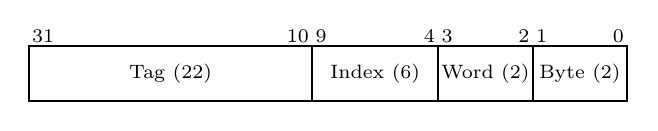
\begin{tikzpicture}[font=\scriptsize]
\draw[thick] (0,0) rectangle (3.6,0.7) node[midway]{Tag (22)};
\draw[thick] (3.6,0) rectangle (5.2,0.7) node[midway]{Index (6)};
\draw[thick] (5.2,0) rectangle (6.4,0.7) node[midway]{Word (2)};
\draw[thick] (6.4,0) rectangle (7.6,0.7) node[midway]{Byte (2)};
\node[anchor=south west,inner sep=1pt] at (0,0.7) {31}; \node[anchor=south east,inner sep=1pt] at (3.6,0.7) {10};
\node[anchor=south west,inner sep=1pt] at (3.6,0.7) {9}; \node[anchor=south east,inner sep=1pt] at (5.2,0.7) {4};
\node[anchor=south west,inner sep=1pt] at (5.2,0.7) {3}; \node[anchor=south east,inner sep=1pt] at (6.4,0.7) {2};
\node[anchor=south west,inner sep=1pt] at (6.4,0.7) {1}; \node[anchor=south east,inner sep=1pt] at (7.6,0.7) {0};
\end{tikzpicture}
\caption{32-bit byte-address partition used by the decoder.}\label{fig:addr}
\end{figure}

Table~\ref{tab:ex} gives worked examples taken from the integrated test. Addresses \texttt{0x000}, \texttt{0x400} and \texttt{0x804} all map to index~0 but carry different tags (0, 1 and 2), so they evict one another; this is how the conflict-replacement behavior is provoked in simulation.

\begin{table}[!t]
\caption{Worked Address-Decoding Examples}\label{tab:ex}
\centering
\renewcommand{\arraystretch}{1.1}
\begin{tabular}{@{}lcccc@{}}
\toprule
\textbf{Address} & \textbf{Tag} & \textbf{Index} & \textbf{Word} & \textbf{Block base}\\
\midrule
\texttt{0x00000000} & 0 & 0 & 0 & \texttt{0x000}\\
\texttt{0x00000004} & 0 & 0 & 1 & \texttt{0x000}\\
\texttt{0x00000400} & 1 & 0 & 0 & \texttt{0x400}\\
\texttt{0x00000804} & 2 & 0 & 1 & \texttt{0x800}\\
\texttt{0x00000060} & 0 & 6 & 0 & \texttt{0x060}\\
\texttt{0x00000460} & 1 & 6 & 0 & \texttt{0x460}\\
\bottomrule
\end{tabular}
\end{table}

\subsection{Read and Write Operation}\label{sec:rw}
\emph{Read hit:} the controller returns the selected word from the indexed line. \emph{Read miss:} it requests the aligned 16-byte block from main memory, waits for the memory-ready response, installs the returned block and tag, marks the line valid and returns the requested word. \emph{Write hit:} the selected cache word is updated and the same word is written to main memory; completion is reported after the memory acknowledgement. \emph{Write miss:} the controller first fetches and installs the containing block, updates the selected word, writes that word through to main memory and then completes the request. Because every write is propagated to memory, no dirty bits are required.

\subsection{Controller Microarchitecture}\label{sec:fsm}
The controller is an FSM with eight states (Fig.~\ref{fig:fsm}): \texttt{IDLE}, \texttt{LOOKUP}, \texttt{REFILL\_WAIT}, \texttt{REFILL\_INSTALL}, \texttt{READ\_MISS\_RETURN}, \texttt{WRITE\_HIT\_WAIT}, \texttt{WRITE\_MISS\_UPDATE} and \texttt{WRITE\_MISS\_WAIT}. In \texttt{IDLE} the controller captures a new request. \texttt{LOOKUP} determines hit or miss: a read hit returns data directly, while a write hit updates the cache word and issues a memory write. A miss requests a block refill and waits for memory. After refill the block is installed; a read miss then returns the selected word, whereas a write miss updates the selected word and issues a write-through transaction.

The processor protocol allows one outstanding request. Requests presented while the controller is busy are not queued, and the requester must deassert \texttt{cpu\_req} for at least one rising clock edge between transactions. The controller produces a one-cycle \texttt{cpu\_ready} completion pulse. The registered events \texttt{access\_complete}, \texttt{hit\_event} and \texttt{miss\_event} identify completed requests; exactly one of hit or miss accompanies each completion.

Table~\ref{tab:states} lists the state encodings, which are exposed on the \texttt{controller\_state} output for waveform inspection.

\begin{table}[!t]
\caption{Controller States and Actions}\label{tab:states}
\centering
\renewcommand{\arraystretch}{1.1}
\footnotesize
\begin{tabular}{@{}clp{4.5cm}@{}}
\toprule
\textbf{Code} & \textbf{State} & \textbf{Action}\\
\midrule
0 & \texttt{IDLE} & Wait for \texttt{cpu\_req}; latch address, operation and write data\\
1 & \texttt{LOOKUP} & Evaluate hit/miss; complete a read hit; start a write hit or a refill\\
2 & \texttt{REFILL\_WAIT} & Hold block request until \texttt{mem\_ready}\\
3 & \texttt{REFILL\_INSTALL} & Install 128-bit block, tag and valid bit\\
4 & \texttt{READ\_MISS\_RETURN} & Return the requested word; report a miss\\
5 & \texttt{WRITE\_HIT\_WAIT} & Wait for write-through acknowledgement; report a hit\\
6 & \texttt{WRITE\_MISS\_UPDATE} & Update the selected word; issue write-through\\
7 & \texttt{WRITE\_MISS\_WAIT} & Wait for acknowledgement; report a miss\\
\bottomrule
\end{tabular}
\end{table}

\begin{figure*}[!t]
\centering
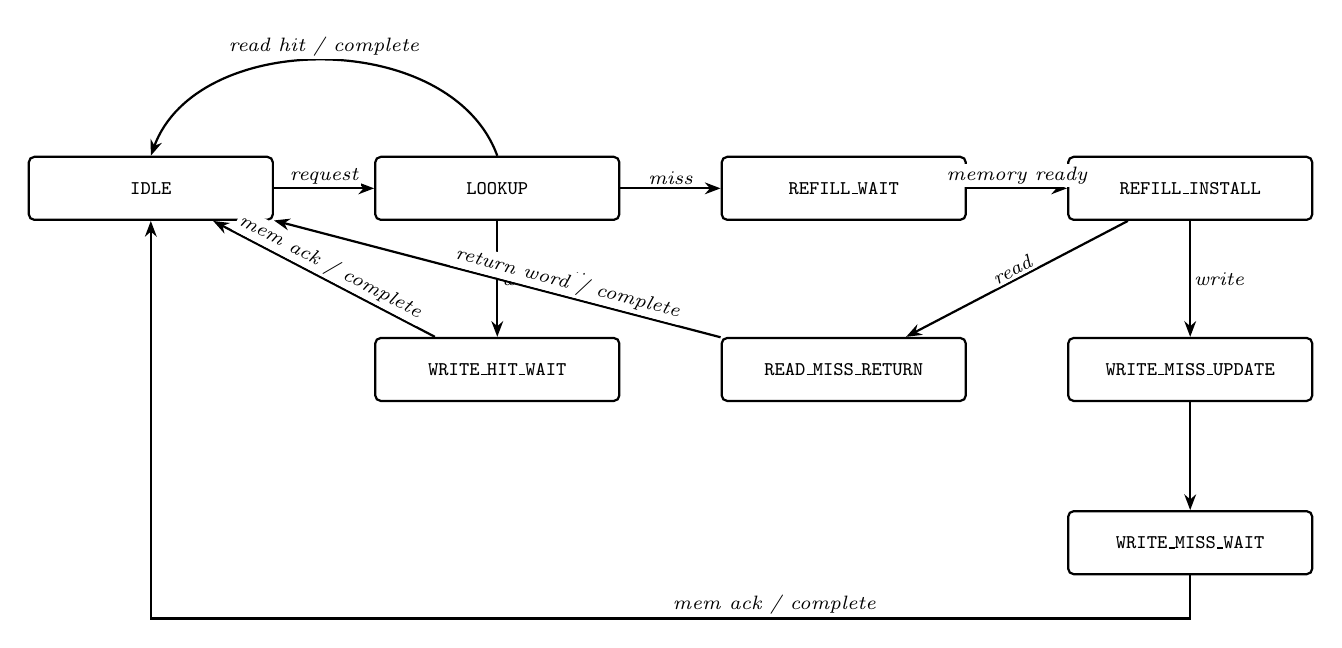
\begin{tikzpicture}
\node[st] (idle) at (0,0) {IDLE};
\node[st] (look) at (4.4,0) {LOOKUP};
\node[st] (rw) at (8.8,0) {REFILL\_WAIT};
\node[st] (ri) at (13.2,0) {REFILL\_INSTALL};
\node[st] (whw) at (4.4,-2.3) {WRITE\_HIT\_WAIT};
\node[st] (rmr) at (8.8,-2.3) {READ\_MISS\_RETURN};
\node[st] (wmu) at (13.2,-2.3) {WRITE\_MISS\_UPDATE};
\node[st] (wmw) at (13.2,-4.5) {WRITE\_MISS\_WAIT};
\draw[arr] (idle) -- node[lab,above]{request} (look);
\draw[arr] (look) -- node[lab,above]{miss} (rw);
\draw[arr] (rw) -- node[lab,above]{memory ready} (ri);
\draw[arr] (look) -- node[lab,right]{write hit} (whw);
\draw[arr] (ri) -- node[lab,above,sloped]{read} (rmr);
\draw[arr] (ri) -- node[lab,right]{write} (wmu);
\draw[arr] (wmu) -- (wmw);
\draw[arr] (look.north) to[out=110,in=70] node[lab,above]{read hit / complete} (idle.north);
\draw[arr] (whw) -- node[lab,above,sloped]{mem ack / complete} (idle);
\draw[arr] (rmr) -- node[lab,above,sloped,pos=0.35]{return word / complete} (idle);
\draw[arr] (wmw.south) -- ++(0,-0.55) -| node[lab,above,pos=0.2]{mem ack / complete} (idle.south);
\end{tikzpicture}
\caption{Controller FSM paths for read hits, misses and write-through operations. The controller returns to \texttt{IDLE} after the completion pulse; write operations complete after the memory acknowledgement.}\label{fig:fsm}
\end{figure*}

%%%%%%%%%%%%%%%%%%%% IV %%%%%%%%%%%%%%%%%%%%
\section{Implementation}\label{sec:impl}
\subsection{Module Hierarchy}\label{sec:mods}
The implemented hierarchy contains five leaf modules (about 650 lines of Verilog in total) integrated by \texttt{cache\_top}; Table~\ref{tab:mods} lists them. All sequential modules share \texttt{clk} and a synchronous active-high \texttt{reset}.

\begin{table}[!t]
\caption{RTL Modules and Source Files}\label{tab:mods}
\centering
\renewcommand{\arraystretch}{1.1}
\begin{tabular}{@{}lp{4.1cm}@{}}
\toprule
\textbf{Module} & \textbf{File}\\
\midrule
Address decoder & \texttt{rtl/address\_decoder.v}\\
Cache storage & \texttt{rtl/cache\_storage.v}\\
Cache controller & \texttt{rtl/cache\_controller.v}\\
Performance monitor & \texttt{rtl/performance\_monitor.v}\\
Main-memory model & \texttt{memory/main\_memory\_model.v}\\
Integrated top level & \texttt{rtl/cache\_top.v}\\
\bottomrule
\end{tabular}
\end{table}

The \emph{decoder} is combinational: it extracts the address fields and performs a 22-bit tag comparison qualified by the stored valid bit, so that
\begin{equation}
\mathrm{hit} = \mathrm{stored\_valid}\;\wedge\;(\mathrm{stored\_tag}=A[31{:}10]).
\label{eq:hit}
\end{equation}
\emph{Cache storage} contains 64 lines, each with a valid bit, a 22-bit tag and 128 data bits; lookup is combinational, refill and word updates are synchronous, reset invalidates every line, and a refill takes priority over a simultaneous word write. The \emph{controller} is sequential RTL that latches the request address, operation and write data on acceptance and drives storage, memory and monitor interfaces with registered one-cycle pulses.

\subsection{Main-Memory Model and Performance Monitor}\label{sec:memmon}
The main-memory model is behavioral and intended for simulation. It contains 4096 32-bit words (16~KiB), initializes all words to zero, optionally loads hexadecimal contents through \texttt{\$readmemh}, supports configurable latency (default five cycles), returns four consecutive words on a block read and supports a 32-bit word write. Reset clears protocol state but does not erase memory contents. The initialization file is a simulation feature and is not part of a synthesizable physical memory macro.

The synthesizable performance monitor uses three 32-bit counters (\texttt{total\_accesses}, \texttt{total\_hits}, \texttt{total\_misses}) with synchronous reset. It increments only when \texttt{access\_complete} is high and exactly one of \texttt{hit\_event} or \texttt{miss\_event} is asserted, so that
\begin{equation}
\mathrm{total\_accesses} = \mathrm{total\_hits} + \mathrm{total\_misses}
\label{eq:inv}
\end{equation}
holds between counter wraparounds. Internal refill and write-through memory operations are not counted as separate processor accesses.

\subsection{Top-Level Interface}\label{sec:iface}
The integrated module \texttt{cache\_top} exposes the processor-side interface and the performance counters, and parameters \texttt{MEM\_WORDS} (4096) and \texttt{MEM\_LATENCY} (5) for the embedded memory model (Table~\ref{tab:ports}). Internally, the controller drives the memory with a request, a write-enable, a byte address, 32-bit write data and receives a \texttt{ready} strobe and a 128-bit block.

\begin{table}[!t]
\caption{\texttt{cache\_top} Ports}\label{tab:ports}
\centering
\renewcommand{\arraystretch}{1.05}
\footnotesize
\begin{tabular}{@{}llcp{3.0cm}@{}}
\toprule
\textbf{Signal} & \textbf{Dir.} & \textbf{Bits} & \textbf{Description}\\
\midrule
\texttt{clk}, \texttt{reset} & in & 1 & Clock; sync.\ reset\\
\texttt{cpu\_req} & in & 1 & Request (one outstanding)\\
\texttt{cpu\_write} & in & 1 & 1 = write, 0 = read\\
\texttt{cpu\_addr} & in & 32 & Aligned word address\\
\texttt{cpu\_wdata} & in & 32 & Write data\\
\texttt{cpu\_ready} & out & 1 & One-cycle completion\\
\texttt{cpu\_rdata} & out & 32 & Read data with ready\\
\texttt{total\_accesses} & out & 32 & Completed accesses\\
\texttt{total\_hits} & out & 32 & Hit counter\\
\texttt{total\_misses} & out & 32 & Miss counter\\
\texttt{controller\_state} & out & 4 & FSM state (debug)\\
\bottomrule
\end{tabular}
\end{table}

%%%%%%%%%%%%%%%%%%%% V %%%%%%%%%%%%%%%%%%%%
\section{Verification and Results}\label{sec:ver}
\subsection{Verification Methodology}\label{sec:meth}
Each module has a self-checking Verilog testbench, and a top-level testbench instantiates the real \texttt{cache\_top} with the actual decoder, storage, controller, memory and monitor. Simulations are compiled with Icarus Verilog \cite{icarus} (\texttt{iverilog -g2012 -Wall}) and executed with \texttt{vvp}. In the integrated test, memory is seeded with the deterministic pattern \texttt{0x600d0000 + word\_index}, so every returned word can be checked against a known value. The regression is run from the repository root with a single script (\texttt{sim/run\_krishna\_tests.sh}), which runs all unit benches, the integrated bench and the eight waveform scenarios. The final run completed with every suite passing.

\subsection{Unit-Level Results}\label{sec:unit}
Table~\ref{tab:unit} summarizes the unit-level regression. The address-decoder bench alone executes ten suites and 374 checks, including a full 64-index sweep, all four word offsets, valid/tag combinations, walking-one/zero isolation of all 22 tag bits and 200 randomized vectors checked against a reference model. The controller bench exercises cold miss and four-word refill, repeated hits, conflicting-tag replacement, write hit, write miss and a dropped busy request, and ends with 13 accesses classified as 7 hits and 6 misses. The memory bench confirms a four-word block read, exact-word write, read-after-write and a measured response wait of five cycles. The memory-initialization bench confirms that \texttt{\$readmemh} contents appear in ascending address order; Icarus emits a sparse-file warning because the sample file holds four words rather than 4096, and the remaining locations stay zero.

\begin{table}[!t]
\caption{Unit-Level Verification Results}\label{tab:unit}
\centering
\renewcommand{\arraystretch}{1.1}
\begin{tabular}{@{}lp{4.3cm}c@{}}
\toprule
\textbf{Testbench} & \textbf{Result} & \textbf{Status}\\
\midrule
Address decoder & 10 suites, 374 checks, 0 errors & Pass\\
Cache storage & Reset, refill, word select/update, refill priority & Pass\\
Controller & 13 accesses: 7 hits, 6 misses & Pass\\
Main memory & Block read, write, read-after-write, 5-cycle latency & Pass\\
Memory init. & \texttt{\$readmemh} order verified & Pass\\
Perf.\ monitor & 10 tests, invariant \eqref{eq:inv} held & Pass\\
\bottomrule
\end{tabular}
\end{table}

\subsection{Integrated Results and Waveform Scenarios}\label{sec:integ}
The combined integrated sequence passed \textbf{39 checks with 0 failures} over 26 completed processor accesses, with the monitor reporting 13 hits and 13 misses, matching the expected counts exactly. In addition, eight isolated runs reset the design and counters and dump a VCD waveform each (Table~\ref{tab:scen}). Every run passed and its counters matched expectation (Table~\ref{tab:cnt}). The VCD files include clock/reset, processor request and response signals, controller state, performance counters, memory request/response/address/block data, and cache refill and word-write controls.

\begin{table}[!t]
\caption{Isolated Waveform Scenarios}\label{tab:scen}
\centering
\renewcommand{\arraystretch}{1.1}
\begin{tabular}{@{}p{3.4cm}p{3.3cm}c@{}}
\toprule
\textbf{Scenario} & \textbf{Behavior demonstrated} & \textbf{Chk.}\\
\midrule
\texttt{reset\_invalid\_lines} & Valid bits clear; first read misses & 5\\
\texttt{cache\_miss} & Cold miss returns memory data & 5\\
\texttt{cache\_hit} & Repeat access hits & 6\\
\texttt{consecutive\_requests} & Protocol-legal back-to-back reads & 7\\
\texttt{controller\_busy} & Busy request dropped, not queued & 6\\
\texttt{block\_refill\_order} & Words 0--3 in ascending order & 9\\
\texttt{conflict\_replacement} & Same-index eviction, no stale data & 9\\
\texttt{write\_through} & Write hit/miss visible in cache and memory & 12\\
\bottomrule
\end{tabular}
\end{table}

\begin{table}[!t]
\caption{Performance Counters: Expected vs.\ Actual}\label{tab:cnt}
\centering
\renewcommand{\arraystretch}{1.1}
\begin{tabular}{@{}lccc@{}}
\toprule
\textbf{Run} & \textbf{Acc.} & \textbf{Hits} & \textbf{Miss}\\
\midrule
Full combined sequence & 26 & 13 & 13\\
Reset / invalid lines & 1 & 0 & 1\\
Cache miss & 1 & 0 & 1\\
Cache hit & 2 & 1 & 1\\
Consecutive requests & 3 & 2 & 1\\
Controller busy & 2 & 0 & 2\\
Four-word refill order & 4 & 3 & 1\\
Conflict replacement & 4 & 1 & 3\\
Write-through & 4 & 2 & 2\\
\bottomrule
\end{tabular}\\[2pt]
{\footnotesize Expected and actual values were identical in every run.}
\end{table}

The conflict scenario demonstrates the main weakness of direct mapping: addresses \texttt{0x0} and \texttt{0x400} share index 0 but differ in tag, so each evicts the other. The write-through scenario confirms that a written word appears in both the cache and main memory, that the other three words of the block are unchanged, and that a write miss allocates the block.

\subsection{Waveform Timing Analysis}\label{sec:wave}
The committed VCD files were post-processed to extract the controller state, handshake and completion signals. Fig.~\ref{fig:wavehit} shows the \texttt{cache\_hit} scenario. The first read is a cold miss: the controller captures the request, performs the lookup, issues \texttt{mem\_req}, remains in \texttt{REFILL\_WAIT} for seven cycles (the configured five-cycle memory latency plus two cycles of request/response handshake), installs the block, and returns the word with \texttt{cpu\_ready} and \texttt{miss\_event}. The repeated read then follows the short \texttt{IDLE}\,$\rightarrow$\,\texttt{LOOKUP}\,$\rightarrow$\,\texttt{IDLE} path and raises \texttt{hit\_event} one cycle after the lookup.

Fig.~\ref{fig:wavewt} shows write-through behavior. On the write hit, a memory write (\texttt{mem\_req} with \texttt{mem\_write\_en}) is issued from \texttt{LOOKUP} and the controller waits in \texttt{WRITE\_HIT\_WAIT} until \texttt{mem\_ready}; only then are \texttt{cpu\_ready} and \texttt{hit\_event} asserted. On the write miss the controller first refills the block, then issues the write-through and waits in \texttt{WRITE\_MISS\_WAIT}, completing with \texttt{miss\_event}. Exactly one of \texttt{hit\_event} or \texttt{miss\_event} accompanies each completion in all recorded scenarios.

\begin{figure*}[!t]
\centering
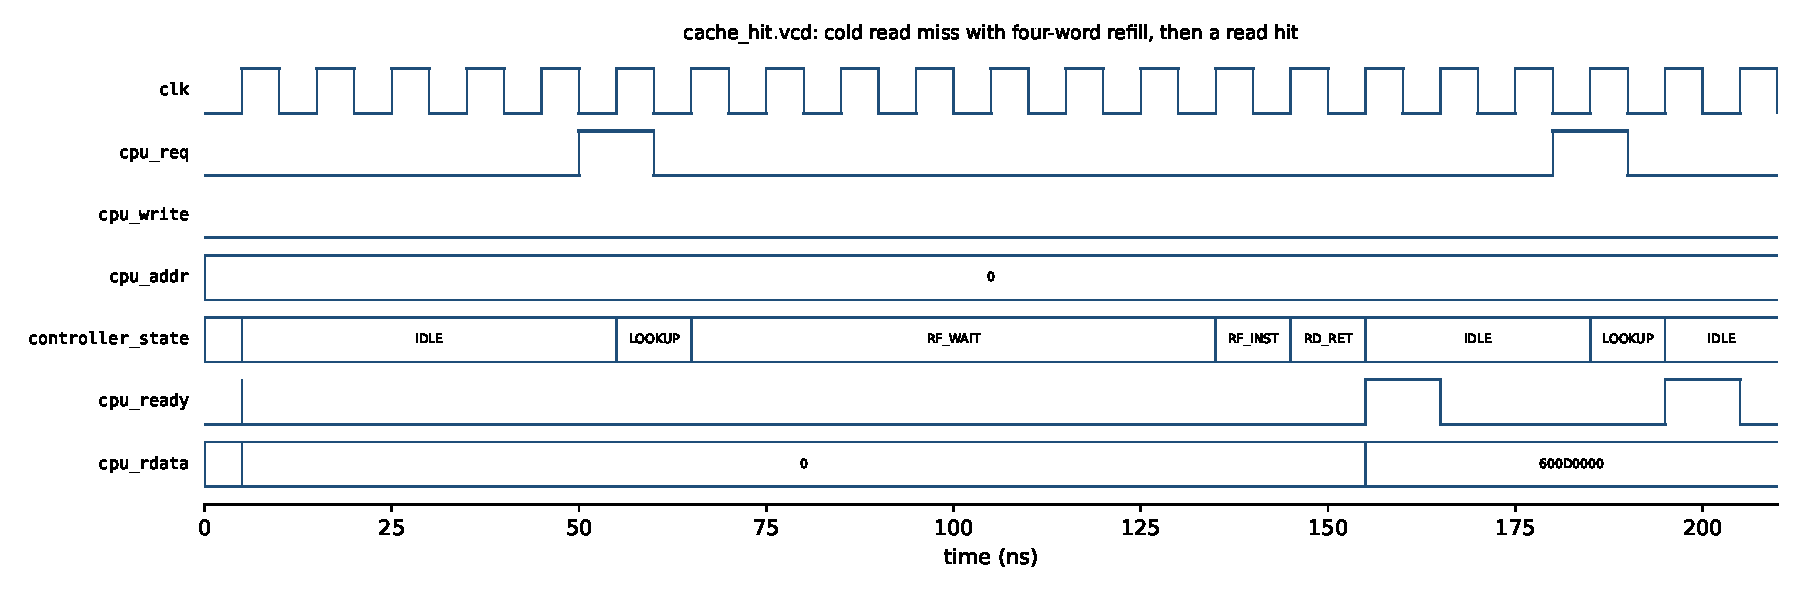
\includegraphics[width=0.92\textwidth]{wave_hit.pdf}
\caption{Waveform extracted from \texttt{cache\_hit.vcd}: a cold read miss with four-word refill followed by a read hit.}\label{fig:wavehit}
\end{figure*}

\begin{figure*}[!t]
\centering
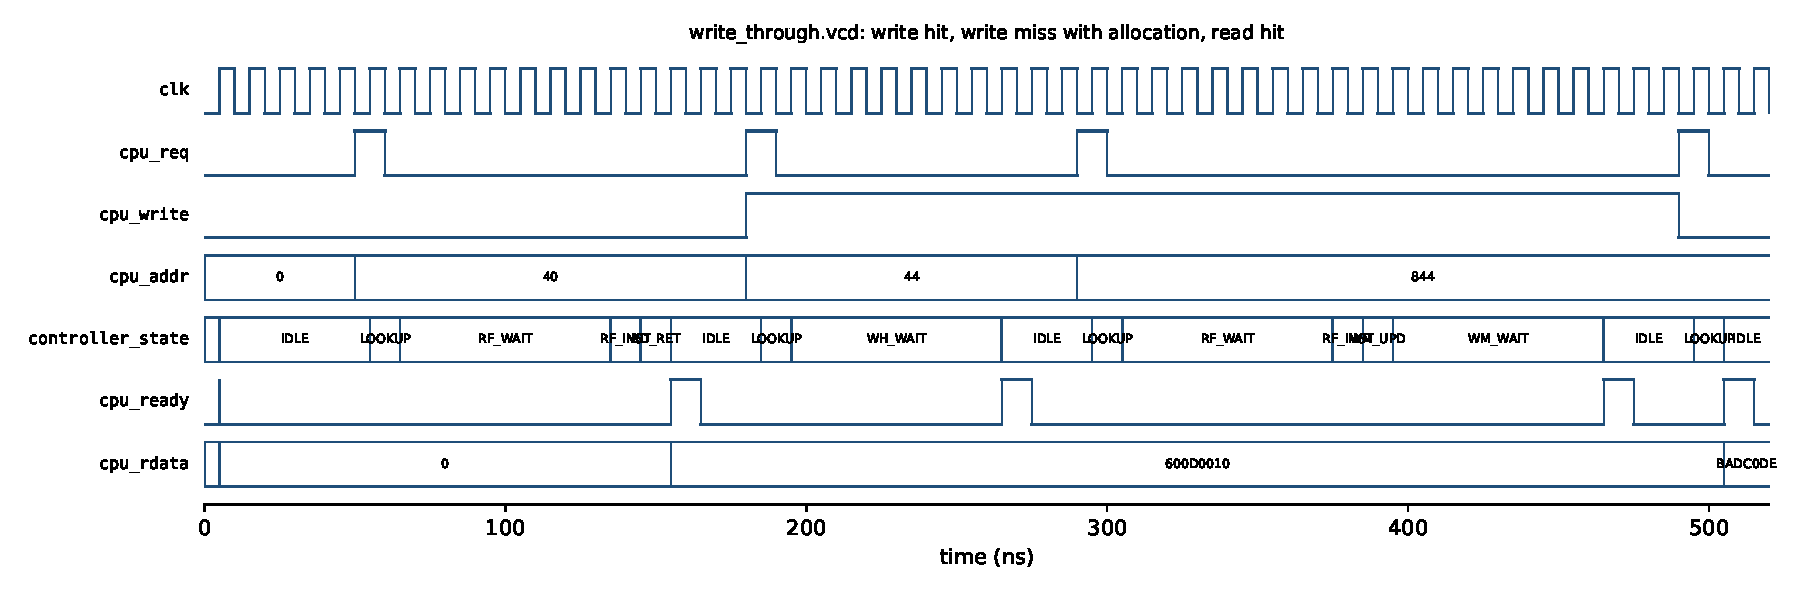
\includegraphics[width=0.92\textwidth]{wave_wt.pdf}
\caption{Waveform extracted from \texttt{write\_through.vcd}: write hit, write miss with allocation, and a read hit to the allocated line.}\label{fig:wavewt}
\end{figure*}

\subsection{Integrated Access Trace}\label{sec:trace}
Table~\ref{tab:trace} lists all 26 accesses of the combined integrated sequence (reads \textbf{R}, writes \textbf{W}; hit \textbf{H}, miss \textbf{M}). It contains 22 reads and 4 writes: 11 read hits, 11 read misses, 2 write hits and 2 write misses. All results match the expected classification enforced by the testbench, and the monitor's final counters (26/13/13) agree with the trace.

\begin{table*}[!t]
\caption{Classified Access Trace of the Integrated Sequence}\label{tab:trace}
\centering
\renewcommand{\arraystretch}{1.05}
\footnotesize
\begin{tabular}{@{}rcclc@{\hspace{1.6em}}rcclc@{}}
\toprule
\textbf{\#} & \textbf{Op} & \textbf{Address} & \textbf{Idx} & \textbf{Res.} & \textbf{\#} & \textbf{Op} & \textbf{Address} & \textbf{Idx} & \textbf{Res.}\\
\midrule
1 & R & \texttt{0x000} & 0 & M & 14 & R & \texttt{0x050} & 5 & M\\
2 & R & \texttt{0x000} & 0 & H & 15 & R & \texttt{0x03C} & 3 & M\\
3 & R & \texttt{0x004} & 0 & H & 16 & R & \texttt{0x030} & 3 & H\\
4 & R & \texttt{0x400} & 0 & M & 17 & R & \texttt{0x034} & 3 & H\\
5 & R & \texttt{0x000} & 0 & M & 18 & R & \texttt{0x038} & 3 & H\\
6 & W & \texttt{0x004} & 0 & H & 19 & R & \texttt{0x060} & 6 & M\\
7 & R & \texttt{0x004} & 0 & H & 20 & R & \texttt{0x460} & 6 & M\\
8 & W & \texttt{0x804} & 0 & M & 21 & R & \texttt{0x460} & 6 & H\\
9 & R & \texttt{0x804} & 0 & H & 22 & R & \texttt{0x060} & 6 & M\\
10 & R & \texttt{0x010} & 1 & M & 23 & R & \texttt{0x040} & 4 & M\\
11 & R & \texttt{0x014} & 1 & H & 24 & W & \texttt{0x044} & 4 & H\\
12 & R & \texttt{0x018} & 1 & H & 25 & W & \texttt{0x844} & 4 & M\\
13 & R & \texttt{0x020} & 2 & M & 26 & R & \texttt{0x844} & 4 & H\\
\bottomrule
\end{tabular}
\end{table*}

\subsection{Requirements Traceability}\label{sec:trace2}
Table~\ref{tab:req} maps each design requirement to the evidence that exercises it.

\begin{table}[!t]
\caption{Requirement-to-Evidence Mapping}\label{tab:req}
\centering
\renewcommand{\arraystretch}{1.05}
\footnotesize
\begin{tabular}{@{}p{3.1cm}p{4.5cm}@{}}
\toprule
\textbf{Requirement} & \textbf{Evidence}\\
\midrule
64-line index mapping & Decoder index sweep (0--63)\\
Hit = valid $\wedge$ tag match & Decoder tests 4--7; tag-bit isolation\\
Reset invalidates lines & Storage reset test; \texttt{reset\_invalid\_lines}\\
Four-word block order & \texttt{block\_refill\_order}; memory block read\\
Direct-mapped replacement & \texttt{conflict\_replacement}; trace \#4--5, \#20--22\\
Write-through, write-allocate & \texttt{write\_through}; trace \#6, \#8, \#24--25\\
One outstanding request & \texttt{controller\_busy} (dropped request)\\
Hit/miss accounting & Monitor tests; counters 26/13/13\\
\bottomrule
\end{tabular}
\end{table}

%%%%%%%%%%%%%%%%%%%% VI %%%%%%%%%%%%%%%%%%%%
\section{Performance Analysis}\label{sec:perf}
\subsection{Hit and Miss Rates}\label{sec:hit}
For the integrated directed sequence, 26 completed processor accesses were recorded: 13 hits and 13 misses. The sequence-specific rates are
\begin{equation}
H=\frac{13}{26}\times 100 = 50\%,\qquad M = 50\%.
\label{eq:hit_rate}
\end{equation}
These values describe the test sequence only; the sequence deliberately mixes cold misses, conflicts and writes, and is not a workload benchmark; the trace-driven benchmark of Section~\ref{sec:bench} addresses locality.

\subsection{Measured Completion Latency}\label{sec:lat}
Latency $L$ is defined as the number of rising clock edges from the request-capture edge (\texttt{IDLE}$\rightarrow$\texttt{LOOKUP}) up to and including the edge on which \texttt{cpu\_ready} is registered. It was measured from the recorded waveforms with the 10~ns testbench clock and the default five-cycle memory latency, and was identical in every scenario that exercised the same access type (Table~\ref{tab:lat}).

\begin{table}[!t]
\caption{Measured Completion Latency per Access Type}\label{tab:lat}
\centering
\renewcommand{\arraystretch}{1.05}
\footnotesize
\begin{tabular}{@{}lccp{3.1cm}@{}}
\toprule
\textbf{Access} & \textbf{Cycles} & \textbf{ns} & \textbf{State path}\\
\midrule
Read hit & 2 & 20 & \texttt{LOOKUP}\\
Read miss & 11 & 110 & \texttt{LOOKUP}, \texttt{REFILL\_WAIT}, \texttt{REFILL\_INSTALL}, \texttt{READ\_MISS\_RETURN}\\
Write hit & 9 & 90 & \texttt{LOOKUP}, \texttt{WRITE\_HIT\_WAIT}\\
Write miss & 18 & 180 & \texttt{LOOKUP}, \texttt{REFILL\_WAIT}, \texttt{REFILL\_INSTALL}, \texttt{WRITE\_MISS\_UPDATE}, \texttt{WRITE\_MISS\_WAIT}\\
\bottomrule
\end{tabular}
\end{table}

The miss penalty for reads is therefore $11-2=9$ cycles, dominated by the seven-cycle refill wait. Because the cache is write-through, a write hit still costs 9 cycles (4.5$\times$ a read hit), and a write miss costs 18 cycles since it pays for both the refill and the memory write.

\subsection{Average Access Time}\label{sec:amat}
The standard model for the effect of the cache on latency is \cite{hennessy}
\begin{equation}
\mathrm{AMAT} = t_{\mathrm{hit}} + m\cdot t_{\mathrm{penalty}}.
\label{eq:amat}
\end{equation}
With the measured read latencies, $t_{\mathrm{hit}}=2$ and $t_{\mathrm{penalty}}=9$ cycles, so for reads
\begin{equation}
\mathrm{AMAT}_{\mathrm{read}} = 2 + 9(1-H) = 11 - 9H \ \text{cycles},
\label{eq:amat_read}
\end{equation}
plotted in Fig.~\ref{fig:amat}. The 22 reads of the integrated sequence have $H=11/22=50\%$, giving 6.5 cycles. Weighting all 26 accesses by their measured latency from Table~\ref{tab:lat} gives a total service time of
\begin{equation}
11{\cdot}2 + 11{\cdot}11 + 2{\cdot}9 + 2{\cdot}18 = 197\ \text{cycles},
\end{equation}
an average of $197/26 \approx 7.6$ cycles per access. This figure is derived from the measured per-type latencies rather than from a single end-to-end simulation, and it excludes idle gaps between requests.

\begin{figure}[!t]
\centering
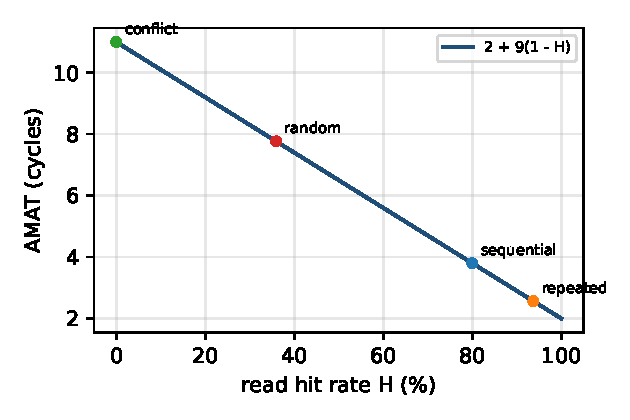
\includegraphics[width=0.95\columnwidth]{amat.pdf}
\caption{Analytical average read latency versus read hit rate, using the measured 2-cycle hit and 11-cycle miss latencies.}\label{fig:amat}
\end{figure}


\subsection{Trace-Driven Benchmark}\label{sec:bench}
\textbf{Methodology.} To evaluate locality beyond the directed tests, a trace-driven functional model of the cache was written in Python \cite{script}. It is an architecture-level model, not an RTL simulation, and mirrors the RTL configuration of 64 lines and 16-byte blocks. For each word-aligned byte address, the block number is $\lfloor A/16\rfloor$, the index is the block number modulo 64 and the tag is $\lfloor \text{block}/64\rfloor$. Each workload starts with all valid bits clear; a hit requires a valid indexed line with a matching tag, and a miss installs the requested tag. The hit rate is hits divided by reads, and the analytical average memory access time is Eq.~\eqref{eq:amat} with the idealized assumptions $t_{\mathrm{hit}}=1$ cycle and $t_{\mathrm{penalty}}=5$ cycles (the configured main-memory response latency). The traces are read-only, so write-through behavior is not exercised. The trace dataset \cite{traces} contains the four workloads in Table~\ref{tab:traces}; the random workload is generated by \path{analysis/gen_random_trace.py} with seed 2026.

\textbf{RTL replay.} The same traces are also replayed through \texttt{cache\_top} by \path{sim/testbenches/tb_trace_replay.v}. Each workload runs from reset, every memory word is preloaded with a distinct pattern so that a wrong word or stale line shows up as a data error, and the cycles from the request edge to \texttt{cpu\_ready} are counted for every access. Hit and miss counts are read from the hardware performance counters. The measured AMAT is total cycles divided by accesses.

\begin{table}[!t]
\caption{Benchmark Workloads and Simulated Hit/Miss Counts}\label{tab:traces}
\centering
\renewcommand{\arraystretch}{1.05}
\footnotesize
\begin{tabular}{@{}lp{3.0cm}ccc@{}}
\toprule
\textbf{Workload} & \textbf{Access pattern} & \textbf{Reads} & \textbf{Hits} & \textbf{Misses}\\
\midrule
Sequential & Words \texttt{0x00}--\texttt{0x3C} once, then \texttt{0x00}--\texttt{0x0C} again & 20 & 16 & 4\\
Repeated block & Four words at \texttt{0x100}--\texttt{0x10C}, repeated four times & 16 & 15 & 1\\
Conflict thrashing & \texttt{0x000} and \texttt{0x400} alternating (same index, different tags) & 8 & 0 & 8\\
Random & 64 uniform word addresses in \texttt{0x000}--\texttt{0x3FC}, seed 2026 & 64 & 23 & 41\\
\bottomrule
\end{tabular}
\end{table}

\textbf{Results.} The sequential trace misses once per 16-byte block (four cold misses) and then hits on the three remaining words of each block and on the re-read of the first block, illustrating spatial and temporal locality. The repeated-block trace incurs a single cold miss and 15 hits. The conflict trace maps both addresses to index~0, so each access evicts the other and every read misses; this is the pathological case for direct mapping. The random trace touches a working set the size of the cache, so it starts cold and warms as lines are reused, ending at a 35.9\% hit rate. The RTL replay produced exactly the same hit and miss counts as the Python model on all four traces, and every returned word matched memory. Table~\ref{tab:bench} and Fig.~\ref{fig:bench} compare the analytical and measured AMAT.

\begin{table}[!t]
\caption{Trace Benchmark Results}\label{tab:bench}
\centering
\renewcommand{\arraystretch}{1.05}
\footnotesize
\begin{tabular}{@{}lccc@{}}
\toprule
\textbf{Workload} & \textbf{Hit rate} & \textbf{Analytical} & \textbf{Measured (RTL)}\\
\midrule
Sequential & 80\% & 2.00 cycles & 3.80 cycles\\
Repeated block & 93.75\% & 1.3125 cycles & 2.5625 cycles\\
Conflict thrashing & 0\% & 6.00 cycles & 11.00 cycles\\
Random & 35.94\% & 4.20 cycles & 7.77 cycles\\
\bottomrule
\end{tabular}\\[2pt]
\parbox{\columnwidth}{\footnotesize Analytical: $1+5M$ (1-cycle hit, 5-cycle miss penalty). Measured: total cycles over accesses from the RTL replay, which equals $2+9M$.}
\end{table}

\begin{figure}[!t]
\centering
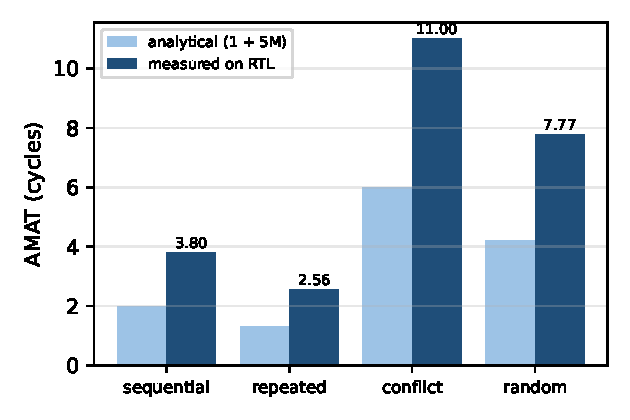
\includegraphics[width=0.95\columnwidth]{bench.pdf}
\caption{Analytical and RTL-measured AMAT for the four benchmark workloads.}\label{fig:bench}
\end{figure}

\textbf{Interpretation and limits.} The analytical column uses the textbook convention and must \emph{not} be read as cycle-accurate: it omits controller state transitions and refill-installation cycles that the waveforms show (a read hit takes 2 cycles and a read miss 11, not 1 and 6). The measured column comes from replaying each trace through \texttt{cache\_top}, and it agrees with Eq.~\eqref{eq:amat_read} evaluated on the measured hit and miss latencies. The traces are small, deliberately constructed patterns that demonstrate spatial locality, temporal locality and conflict misses; they are not a real application workload. No cache-less baseline, CPI, throughput or speedup has been measured, so none is claimed.

%%%%%%%%%%%%%%%%%%%% VII %%%%%%%%%%%%%%%%%%%%
\section{Discussion and Limitations}\label{sec:disc}
\textbf{Design decisions.} Direct mapping was chosen because it needs one tag comparison and no replacement-policy state; write-through with write-allocate removes dirty bits and eviction write-backs, so a replaced line can simply be overwritten. A single-outstanding-request protocol keeps the controller to eight states and makes every access end in exactly one hit or miss event.

\textbf{Limitations.} (i)~Only aligned 32-bit word accesses are supported; byte and half-word writes would require byte enables. (ii)~Requests presented while the controller is busy are dropped, so the processor must retry. (iii)~Without a write buffer, every write stalls for the memory acknowledgement, which the latency measurements show to be the dominant cost for writes. (iv)~The memory is a behavioral simulation model; a synthesized design needs an on-chip block RAM or an external memory controller with its own timing. (v)~The 10~ns testbench clock is faster than the 61.1~MHz the design reaches after place-and-route (Section~\ref{sec:alt}). (vi)~The directed sequence demonstrates correctness, and the trace benchmark uses small constructed read-only traces, so neither establishes real-workload performance. (vii)~The 32-bit counters wrap after $2^{32}$ accesses.

\textbf{Conflict misses.} The trace shows three-way contention at index~0 (addresses \texttt{0x000}, \texttt{0x400}, \texttt{0x804}) and two-way contention at indices~4 and~6. The conflict-thrashing benchmark shows the worst case: a 0\% hit rate for two alternating addresses that share an index. A two-way set-associative organization would hold such pairs simultaneously, at the cost of a second comparator and way-selection logic \cite{patterson,iitkgp}.

%%%%%%%%%%%%%%%%%%%% VIII (alt) %%%%%%%%%%%%%%%%%%%%
\section{Alternative Organizations and Synthesis Results}\label{sec:alt}
Compared with fully associative placement, direct mapping requires only one candidate line and one tag comparison, reducing lookup and replacement complexity; however, it can incur conflict misses when active blocks share an index. Set-associative caches relax this placement restriction but require multiple tag comparisons and way-selection logic \cite{patterson,iitkgp}. Phase~I selected direct mapping to keep the RTL hierarchy and FSM manageable. No quantitative hardware comparison against another implemented cache organization is available.

\textbf{Synthesis.} The design was synthesized with Yosys 0.71 and placed and routed with nextpnr-ecp5 (seed 1, 100~MHz target) for a Lattice ECP5-85F in the CABGA756 package; scripts and logs are in \path{synth/}. For place-and-route the behavioral memory is shrunk to 64 words so it becomes a small stand-in; the cache is unchanged. Table~\ref{tab:synth} lists the results.

\begin{table}[!t]
\caption{ECP5-85F Synthesis and Place-and-Route Results}\label{tab:synth}
\centering
\renewcommand{\arraystretch}{1.05}
\footnotesize
\begin{tabular}{@{}lrrr@{}}
\toprule
\textbf{Resource} & \textbf{Used} & \textbf{Available} & \textbf{\%}\\
\midrule
LUT4 & 18{,}851 & 83{,}640 & 22\\
Flip-flops & 10{,}978 & 83{,}640 & 13\\
Block RAM (DP16KD) & 1 & 208 & $<$1\\
I/O & 201 & 365 & 55\\
\midrule
\multicolumn{4}{@{}l}{Post-route $f_{\max}$: \textbf{61.1~MHz} (100~MHz target not met)}\\
\bottomrule
\end{tabular}
\end{table}

A technology-independent run with the memory as a black box gives 10{,}136 flip-flops, of which 8{,}192 hold the data array and 1{,}408 the tags. The data array reads a whole block in one cycle, so it stays in flip-flops instead of block RAM; the tag array is the only structure inferred as RAM. The critical path starts at that RAM's 5.8~ns clock-to-output and runs through the 22-bit tag compare and the controller next-state logic. Registering the hit decision or banking the data array into four $64\times32$ RAMs would shorten it. An iCE40~HX8K was also tried: the design needs 16{,}467 LUTs against 7{,}680 available, so it does not fit.

%%%%%%%%%%%%%%%%%%%% VIII %%%%%%%%%%%%%%%%%%%%
\section{Individual Contributions}\label{sec:contrib}
The following division is based on module ownership and artifacts recorded in the repository.
\begin{itemize}
\item \textbf{Krishna:} defined the architecture and RTL interface contract; implemented the controller FSM, cache-top wiring, request/response protocol, refill sequencing and write policies.
\item \textbf{Aditya Rana:} implemented the 32-bit address decoder and 22-bit tag comparator; added a self-checking testbench with ten suites and 374 checks, a runner, waveform output and documentation.
\item \textbf{Rachit Gupta:} implemented the 64-line cache storage with tags, valid bits, four-word refill, lookup and selected-word updates; added the cache-storage unit testbench.
\item \textbf{Saumya Mishra:} implemented the behavioral memory model with configurable latency, block reads, word writes and initialization; implemented the synthesizable performance monitor and its unit tests.
\item \textbf{Nishtha Gupta:} added the integrated cache-top testbench, edge-case verification, eight isolated VCD scenarios and the consolidated verification report.
\item \textbf{Trace benchmark and synthesis:} Saumya Mishra added the read-trace dataset and the analytical model; Krishna added the random workload, the RTL trace-replay testbench and the ECP5 synthesis flow.
\end{itemize}

%%%%%%%%%%%%%%%%%%%% IX %%%%%%%%%%%%%%%%%%%%
\section{Conclusion and Future Work}\label{sec:concl}
This Phase~I project delivers a 1~KiB direct-mapped cache with four-word blocks, write-through/write-allocate policies, a behavioral main memory and performance counters. Unit tests cover the decoder, storage, controller, memory and monitor. The integrated test passed 39 checks with no failures across 26 accesses (13 hits, 13 misses), and eight isolated VCD scenarios supplement the directed tests. Waveform measurements show completion latencies of 2, 11, 9 and 18 cycles for a read hit, read miss, write hit and write miss. Four read workloads replayed through the RTL gave hit rates of 80\%, 93.75\%, 0\% and 35.9\% for sequential, repeated-block, conflict-thrashing and random patterns, with measured AMAT of 3.80, 2.56, 11.00 and 7.77 cycles. On a Lattice ECP5-85F the cache uses 22\% of the LUTs and reaches 61.1~MHz. These results confirm the expected behavior: strong spatial and temporal locality benefit, and a worst case when addresses share an index.

Further work includes moving the data array into block RAM to raise $f_{\max}$, benchmarking with real application traces including writes, and a cache-less baseline to quantify CPI and speedup. Byte and unaligned accesses are outside the current prototype contract and are natural extensions, as are a set-associative variant and a write-back policy for comparison.

\appendices
\section{Reproducing the Results}\label{app:repro}
The project is hosted at \url{https://github.com/CosmicMagnetar/MCA_Capstone_Cache}. Icarus Verilog \cite{icarus} must be installed. From the repository root:
\begin{itemize}
\item \path{bash sim/run_krishna_tests.sh} compiles and runs every unit testbench, the integrated bench and all eight waveform scenarios, and ends with ``ALL PHASE I UNIT, INTEGRATION, AND WAVEFORM TESTS COMPLETED''.
\item \path{bash sim/run_cache_top_verification.sh} runs only the integrated and waveform tests.
\item \path{python3 analysis/cache_trace_benchmark.py} runs the trace benchmark \cite{script} on \path{sim/traces/phase1_read_traces.csv} \cite{traces}; \path{--hit-time} and \path{--miss-penalty} override the 1- and 5-cycle assumptions.
\item \path{bash sim/run_trace_benchmark.sh} replays every workload through the RTL and writes \path{docs/results/rtl_trace_results.csv}.
\item \path{bash synth/run_synthesis.sh} reruns synthesis and place-and-route (Yosys and nextpnr-ecp5).
\item \path{python3 report/make_figures.py} regenerates the four figures from the VCDs and the trace results.
\item A single scenario can be run by passing \texttt{+SCENARIO=<name>} to \texttt{vvp}, where \texttt{<name>} is one of the eight scenario names in Table~\ref{tab:scen}.
\end{itemize}
Source files are in \texttt{rtl/} and \texttt{memory/}, testbenches in \texttt{sim/testbenches/}, waveforms and the consolidated verification report in \texttt{sim/waveforms/}, and design notes in \texttt{docs/}.

\section{Summary of Simulation Log}
The final regression log reports: address decoder 374 checks, 0 errors; cache storage all tests passed; controller 13 accesses (7 hits, 6 misses); main memory block read, write, read-after-write and 5-cycle latency passed; memory initialization passed; performance monitor 10 of 10 tests passed; integrated \texttt{cache\_top}: 39 run, 39 passed, 0 failed with counters 26/13/13; and all eight waveform scenarios passed with counters matching expectation.

\begin{thebibliography}{1}\label{sec:refs}
\bibitem{patterson} D.~A. Patterson and J.~L. Hennessy, \emph{Computer Organization and Design: The Hardware/Software Interface}, 5th~ed. Waltham, MA, USA: Morgan Kaufmann, 2013.
\bibitem{arm} Arm Ltd., ``Direct-mapped caches,'' in \emph{Armv7-R Programmer's Guide}. [Online]. Available: \url{https://support.arm.com/documentation/den0042/0100/Caches/Cache-architecture/Direct-mapped-caches}. Accessed: Nov.~13, 2026.
\bibitem{iitkgp} IIT Kharagpur Virtual Labs, ``Direct mapped cache,'' \emph{Computer Organization and Architecture}. [Online]. Available: \url{https://coa-iitkgp.vlabs.ac.in/exp/direct-mapped-cache-design/theory.html}. Accessed: Nov.~13, 2026.
\bibitem{hennessy} J.~L. Hennessy and D.~A. Patterson, \emph{Computer Architecture: A Quantitative Approach}, 4th~ed. San Francisco, CA, USA: Morgan Kaufmann, 2007.
\bibitem{verilog} \emph{IEEE Standard for Verilog Hardware Description Language}, IEEE Std 1364-2005, 2006.
\bibitem{icarus} S.~Williams, ``Icarus Verilog.'' [Online]. Available: \url{https://steveicarus.github.io/iverilog/}. Accessed: Nov.~13, 2026.
\bibitem{script} Team 5bit registers, ``cache\_trace\_benchmark.py: Trace-driven functional model of the 1~KiB direct-mapped cache,'' \texttt{analysis/} directory, MCA Capstone Cache repository, 2026. [Online]. Available: \url{https://github.com/CosmicMagnetar/MCA_Capstone_Cache}
\bibitem{traces} Team 5bit registers, ``phase1\_read\_traces.csv: Sequential, repeated-block and conflict read traces,'' \texttt{sim/traces/} directory, MCA Capstone Cache repository, 2026. [Online]. Available: \url{https://github.com/CosmicMagnetar/MCA_Capstone_Cache}
\end{thebibliography}

\end{document}
